\documentclass[tikz,border=6pt]{standalone}
\usepackage{amsmath}
\usetikzlibrary{arrows.meta,calc,patterns,positioning}
\begin{document}

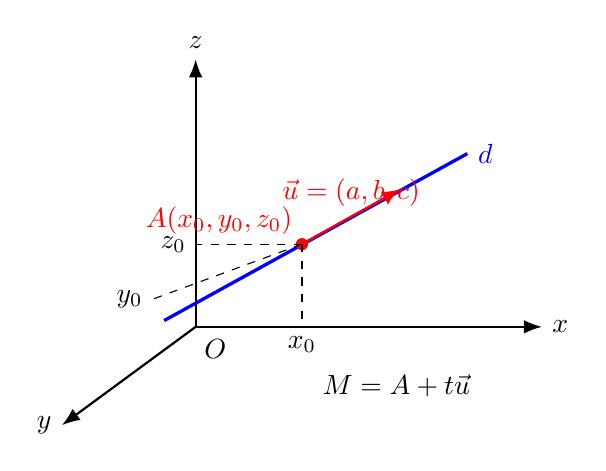
\begin{tikzpicture}[>=Latex,scale=1]
  \coordinate (O) at (0,0);
  \draw[->,thick] (O) -- (4.4,0) node[right] {$x$};
  \draw[->,thick] (O) -- (-1.7,-1.25) node[left] {$y$};
  \draw[->,thick] (O) -- (0,3.4) node[above] {$z$};
  \node at (0.25,-0.28) {$O$};

  \coordinate (A) at (1.35,1.05);
  \coordinate (B) at (3.45,2.2);
  \coordinate (C) at (-0.4,0.08);

  \draw[blue,very thick] (C) -- (B) node[right] {$d$};
  \fill[red] (A) circle (2.2pt) node[above left] {$A(x_0,y_0,z_0)$};
  \draw[->,red,thick] (A) -- ++(1.25,0.7) node[midway,above] {$\vec u=(a,b,c)$};
  \draw[dashed] (A) -- (1.35,0) node[below] {$x_0$};
  \draw[dashed] (A) -- (-0.55,0.35) node[left] {$y_0$};
  \draw[dashed] (A) -- (0,1.05) node[left] {$z_0$};
  \node[align=center] at (2.55,-0.75) {$M=A+t\vec u$};
\end{tikzpicture}

\end{document}
